%!TEX root = ../Thesis.tex
\section{State estimator tuning} % (fold)
\label{sec:state_estimator_tuning}
In this section, the results from the implementation and tuning of the sate estimator are presented. The Kalman filter for position, linear velocity and bias state estimation introduced in section~\ref{ssub:pos_vel_and_bias_state} is implemented in the ROS node "node\_navigation". All measurements are collected in \gls{ROS} bags (data logs) during flight and subsequently used to tune parameters in the state estimator. 

\subsection{Static Landing Pad} % (fold)
\label{sub:static_landing_pad}
\begin{minipage}[c]{0.65\textwidth}
	When tuning the filter for a static landing pad, the prior knowledge of a static landing pad is used to improve the estimates as discussed in~\ref{sub:state_estimation_for_static_landing_pad}. The filter is automatically initialized by adapting the knowledge of using the Landing Pad as takeoff position. The multi marker ArUco tag system is used as fiducial marker and the custom sensor station is used as Landing Pad sensors measurement unit. The filter parameters used in this implementation are given in equation~\ref{eq:filterParamStaticQ} to \ref{eq:filterParamStaticP}
\end{minipage}\hfill
\begin{minipage}[c]{0.3\textwidth}
	\centering
	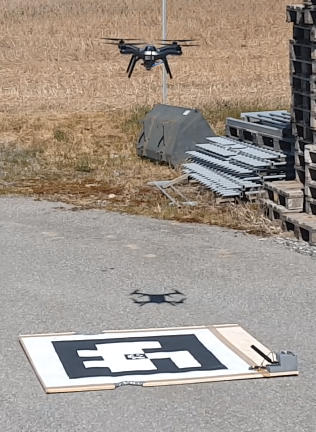
\includegraphics[width=\textwidth]{img/landingStatic.png}
	\captionsetup{type=figure}
	\captionof{figure}{UAV landing on a static Landing Pad}
	\label{fig:landingOnStatic}
\end{minipage}

\begin{align}\label{eq:filterParamStaticQ}
	\vect{Q}_{diag}&=
	\begin{bmatrix}
		 4.1&4.1&4.1&0&0&0&0.1&0.1&10
	\end{bmatrix}\cdot 10^{-3}\\
	\vect{R}_{diag}&=
	\begin{bmatrix}
		2&2&11&0.06&0.06&0.025&10000&10000&10000
	\end{bmatrix}\\\
	\vect{P}_{0,diag}&=
	\begin{bmatrix}
		10&10&10&350&350&380&10&10&10
	\end{bmatrix}\cdot 10^{-3}\label{eq:filterParamStaticP}
\end{align}
where $\vect{Q}_{diag}$, $\vect{R}_{diag}$ and $\vect{P}_{0,diag}$ are the diagonal elements in the corresponding $9\times9$ diagonal matrices.

Figures~\ref{fig:kalmanTuningStaticPos}, \ref{fig:kalmanTuningStaticVel} and \ref{fig:kalmanTuningStaticBias} present the results from the implemented Kalman filter state estimator.
\begin{figure}
\centering
	\begin{subfigure}{.82\textwidth}
		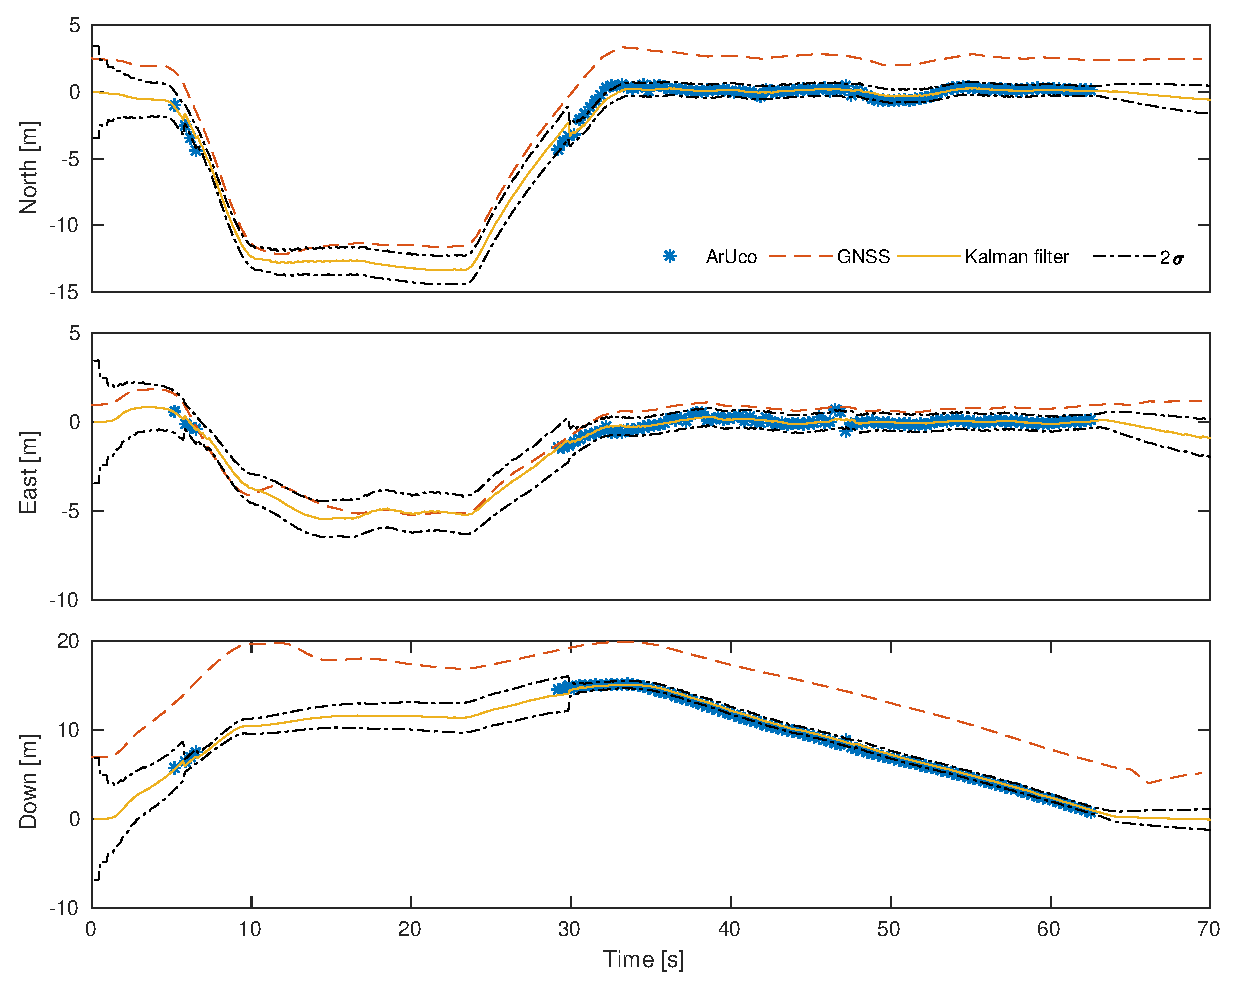
\includegraphics[width=\textwidth]{img/plot/static/kalmanTuningStaticPos.eps}
		\captionof{figure}{State estimates, GNSS- and ArUco measurements of relative position between UAV and LP $\vect{p}^{n}_{l/u}$}
		\label{fig:kalmanTuningStaticPos}
	\end{subfigure}

	\begin{subfigure}{.49\textwidth}
		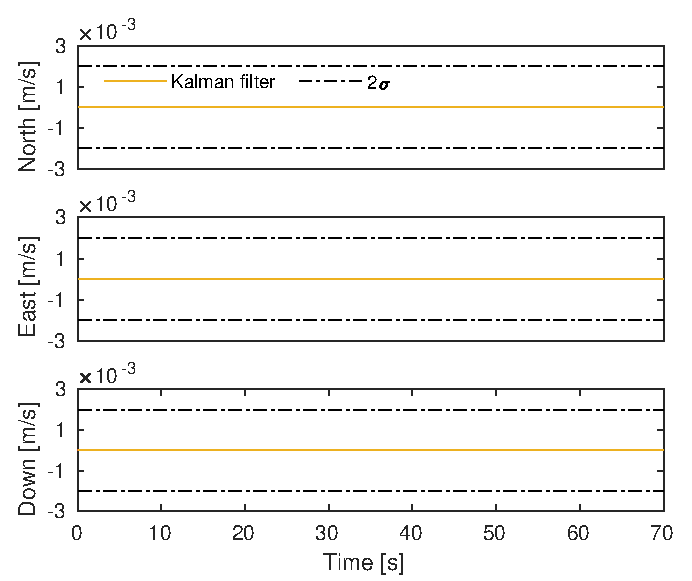
\includegraphics[width=\textwidth]{img/plot/static/kalmanTuningStaticVel.eps}
		\captionof{figure}{State estimates and measurements of the LP velocity $\vect{v}^{n}_{l/n}$}
		\label{fig:kalmanTuningStaticVel}
	\end{subfigure}
	\begin{subfigure}{.49\textwidth}
		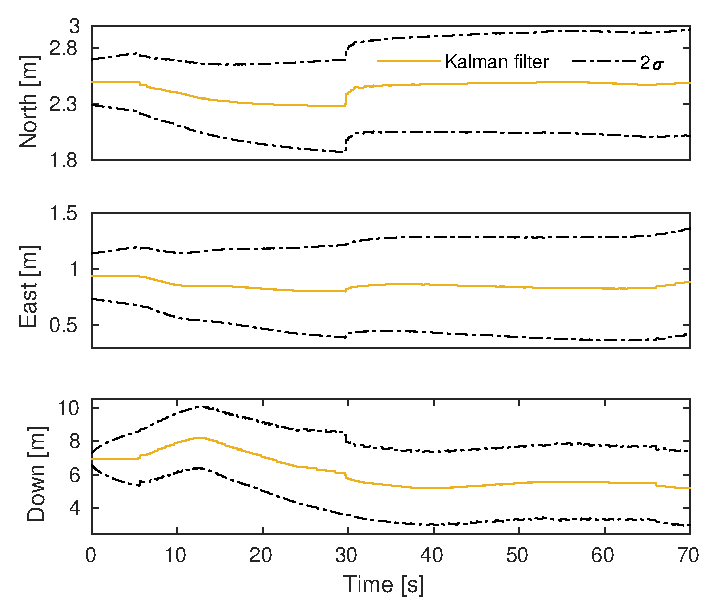
\includegraphics[width=\textwidth]{img/plot/static/kalmanTuningStaticBias.eps}
		\captionof{figure}{State estimates of the position bias $\vect{\beta}^{n}_{l/n}$}
		\label{fig:kalmanTuningStaticBias}
	\end{subfigure}
	\caption{Results from the navigation filter tuned for a static landing pad}\label{fig:kalmanTuningStaticTotal}
\end{figure}
Where sub figure~\ref{fig:kalmanTuningStaticPos} presents the measurements from the ArUco detection, the measurements from the \gls{GNSS} position sensors, estimated relative position vector $\vect{p}^{n}_{l/u}$ and its corresponding $2\sigma$ bound. All given in the North, East and Down components. Moreover, the estimated landing pad velocity $\vect{v}^{n}_{l/n}$ from the same test are given in sub figure~\ref{fig:kalmanTuningStaticVel}. Position bias $\vect{\beta}^{n}_{l/n}$ and its corresponding $2\sigma$ bound are given in \ref{fig:kalmanTuningStaticBias}. The $2 \sigma$ bound represents the 95\% confidence interval.

Figure~\ref{fig:kalmanTuningStaticPosZoom} gives a closed up view of figure~\ref{fig:kalmanTuningStaticPos}.
\begin{figure}
	\centering
	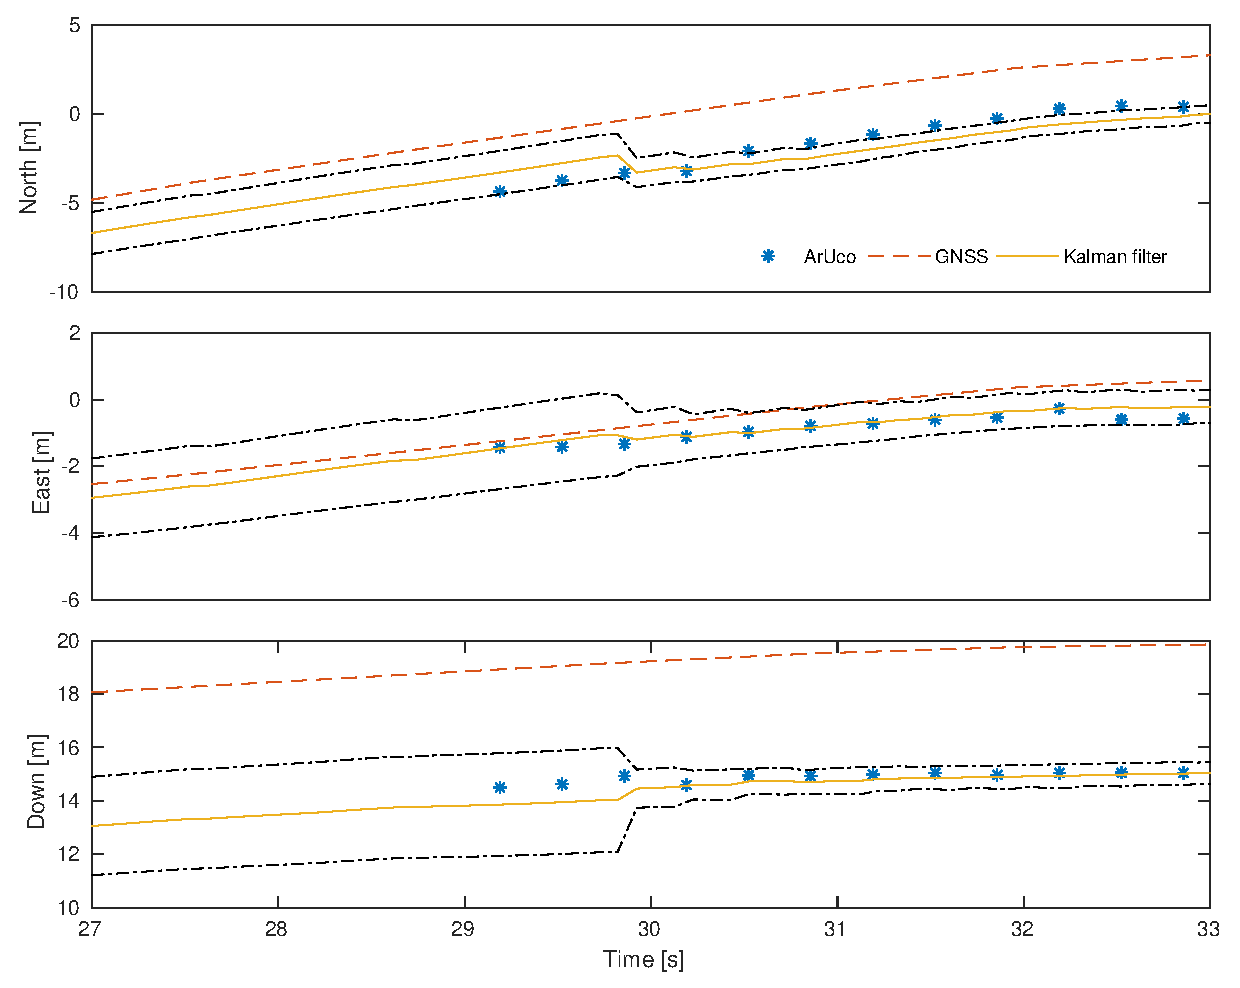
\includegraphics[width=\linewidth]{img/plot/static/kalmanTuningStaticPosZoom.eps}
	\caption{How covariance estimate narrows}{Covariance estimate narrows as the fiducial marker gets within camera sight}
	\label{fig:kalmanTuningStaticPosZoom}
\end{figure}
Moreover, from figure~\ref{fig:kalmanTuningStaticPosZoom} and \ref{fig:kalmanTuningStaticBias} it can be seen how the state estimate corrects, the covariance of the estimate narrows and the estimated bias adjusts as the ArUco tag measurements starts to arrive at $t=29$. 

The figure~\ref{fig:kalmanTuningStaticPos} and~\ref{fig:kalmanTuningStaticPosZoom} illustrates the importance of supplementing the ArUco measurements to the state estimator, in addition to the \gls{GNSS} measurements. Without the presence of ArUco measurements, the position estimate gets higher covariance and navigation biases cannot be updated. 
% subsection static_landing_pad (end)
%From statistic, 95\% of the estimates the $2\sigma$ bound within this bound.

\subsection{Landing Pad in Motion} % (fold)
\label{sub:landing_pad_at_speed}
This section presents the result from the implemented and tuned state estimator in \ref{ssub:pos_and_vel_state}. A multi marker ArUco tag system is placed on the deck of the \gls{FFI} surface vehicle Odin. The already implemented state-of-the-art navigation estimate of the surface vehicle is broadcasted to the \gls{UAV}. The filter parameters used during this tests are given in equation~\ref{eq:filterParamDynamicQ} to \ref{eq:filterParamDynamicP}
\begin{align}\label{eq:filterParamDynamicQ}
	\vect{Q}_{diag}&=
	\begin{bmatrix}
		 4.1&4.1&4.1&10&10&10&0.1&0.1&10
	\end{bmatrix}\cdot 10^{-3}\\
	\vect{R}_{diag}&=
	\begin{bmatrix}
		2&2&11&0.06&0.06&0.025&0.0024&0.0024&0.007
	\end{bmatrix}\\\
	\vect{P}_{0,diag}&=
	\begin{bmatrix}
		140&140&410&12.4&12.4&12.4&28&28&600
	\end{bmatrix}\cdot 10^{-3}\label{eq:filterParamDynamicP}
\end{align}
where $\vect{Q}_{diag}$, $\vect{R}_{diag}$ and $\vect{P}_{0,diag}$ are the diagonal elements in the analogous $9\times9$ diagonal matrices.

As illustrated in figure~\ref{fig:kalmanTuningDynamic7}, the test results was conducted with the \gls{UAV} first hover at a stationary point while the landing pad accelerates up to $1.8m/s$. The \gls{UAV} then starts to fly towards the landing pad and matches its velocity before lovering the altitude and lands on the landing pad.
\begin{figure}
	\centering
	\begin{subfigure}{.75\textwidth}
		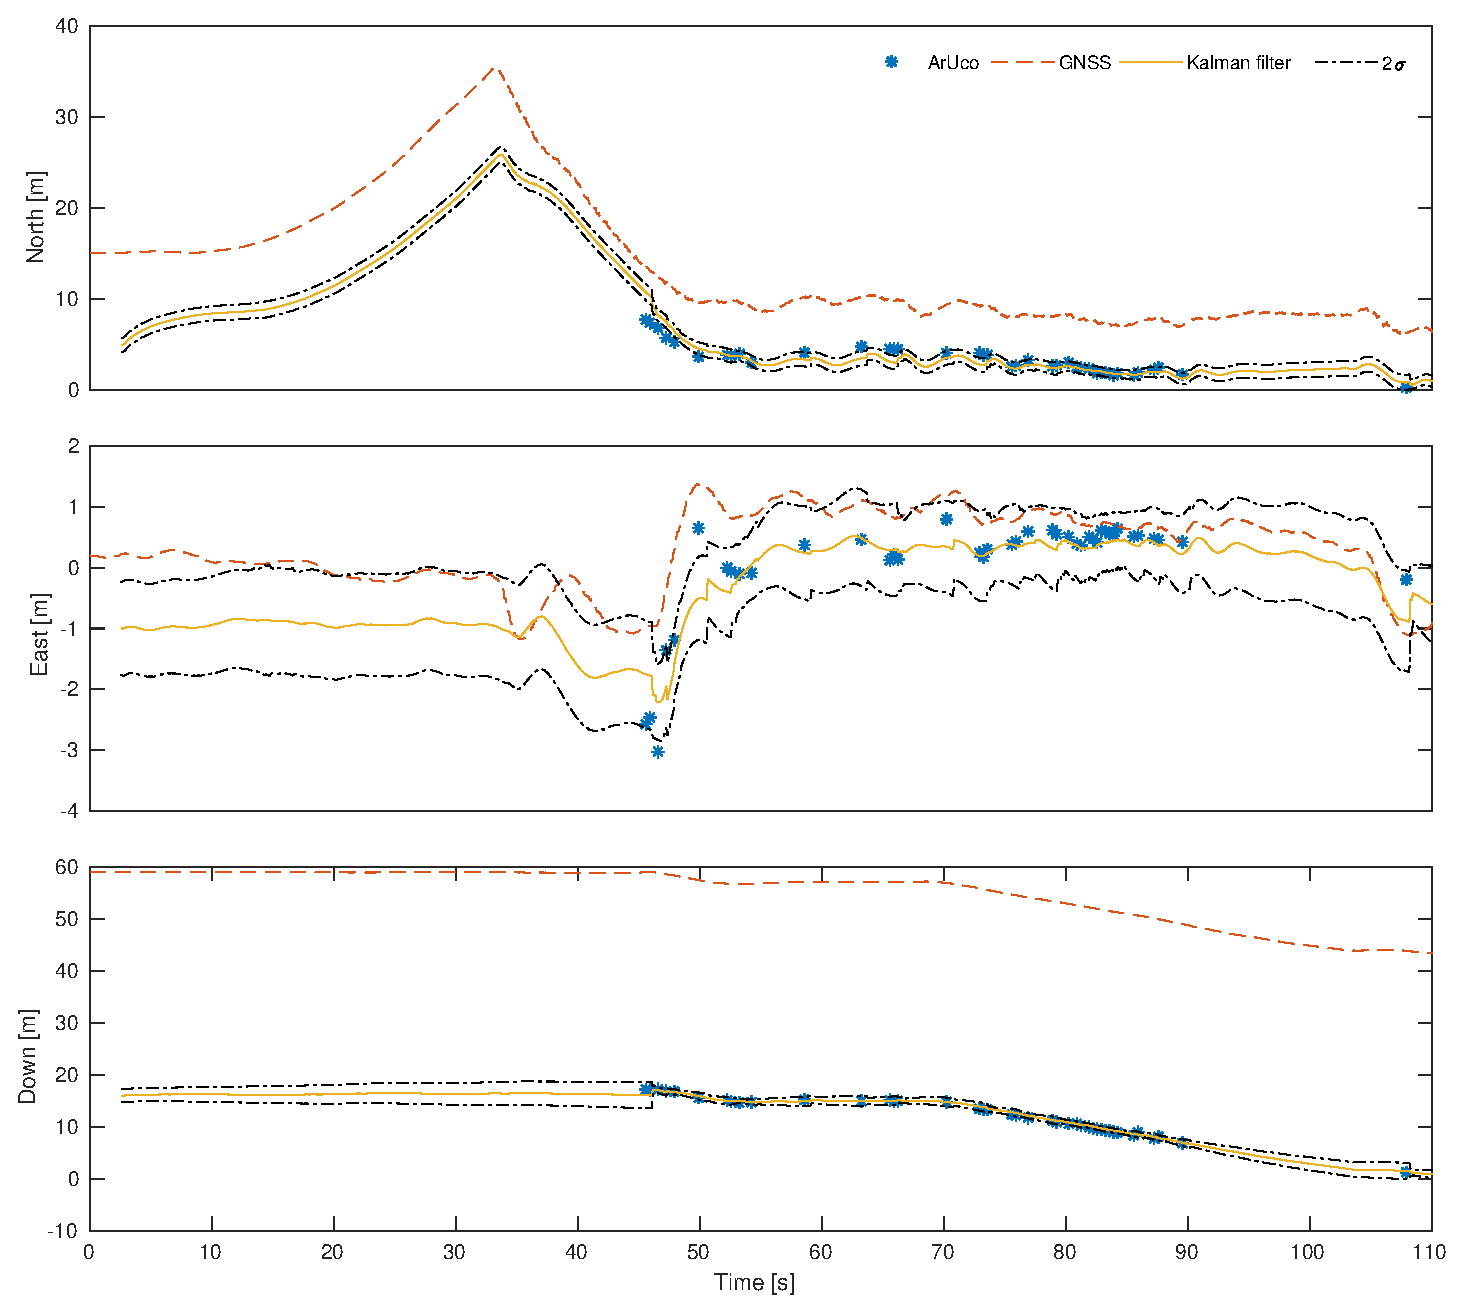
\includegraphics[width=\textwidth]{img/plot/dynamic/dynamic_7_pos.eps}
		\captionof{figure}{State estimates, GNSS- and ArUco measurements of relative position between UAV and LP $\vect{p}^{n}_{l/u}$}
		\label{fig:kalmanTuningDynamic7Pos}
	\end{subfigure}

	\begin{subfigure}{.48\linewidth}
		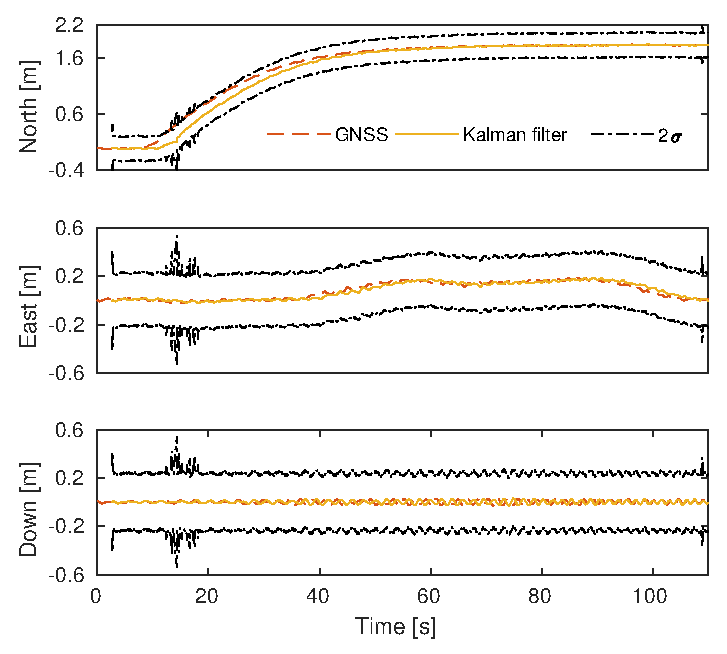
\includegraphics[width=\linewidth]{img/plot/dynamic/dynamic_7_vel.eps}
		\captionof{figure}{State estimates and measurements of the LP velocity $\vect{v}^{n}_{l/n}$}
		\label{fig:kalmanTuningDynamic7Vel}
	\end{subfigure}
	\begin{subfigure}{.48\linewidth}
		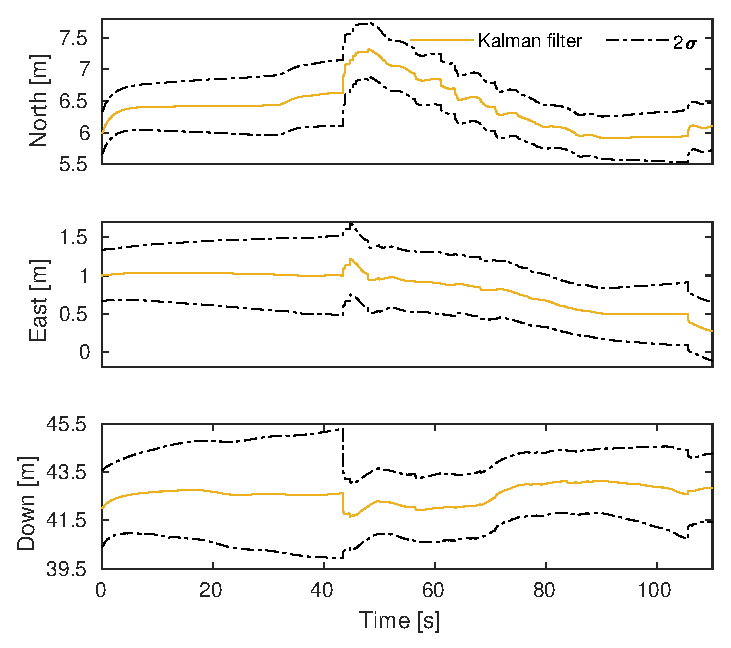
\includegraphics[width=\linewidth]{img/plot/dynamic/dynamic_7_bias.eps}
		\captionof{figure}{Covariance estimate narrows as the fiducial marker gets within camera sight}
		\label{fig:kalmanTuningDynamic7Bias}
	\end{subfigure}
	\caption{Results from the navigation filter tuned for a landing pad at speed}\label{fig:kalmanTuningDynamic7}
\end{figure}
Figure~\ref{fig:kalmanTuningDynamic7closeup} highlights a selection of the ArUco measurements, position estimate and the estimated covariance from figure~\ref{fig:kalmanTuningDynamic7} where the ArUco tag were detectable.
\begin{figure}
	\centering
	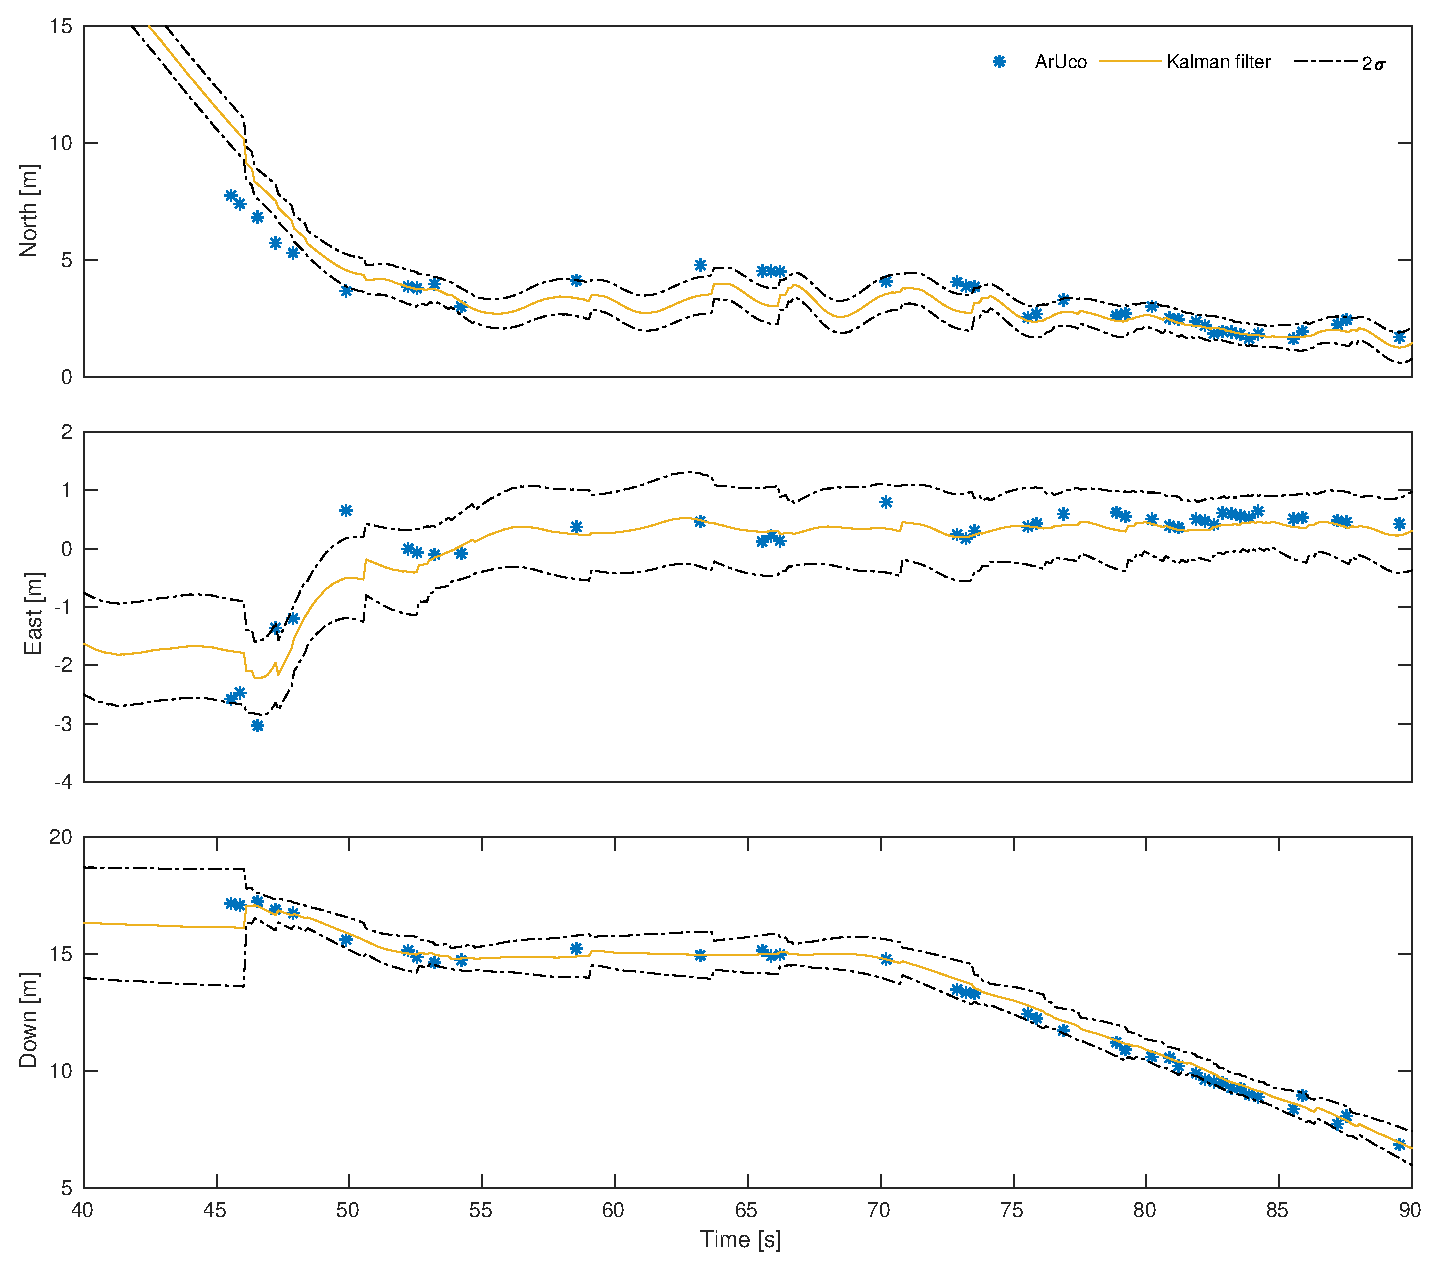
\includegraphics[width=.75\linewidth]{img/plot/dynamic/dynamic_7_closeup.eps}
	\caption{Closeup of the ArUco measurements}{Closeup of the ArUco measurements, estimated position vector $\vect{p}^{n}_{l/u}$ and $2\sigma$ bound during camera fix}
	\label{fig:kalmanTuningDynamic7closeup}
\end{figure}
As figure~\ref{fig:kalmanTuningDynamic7} and \ref{fig:kalmanTuningDynamic7closeup} illustrates, the UAV was oscillating back and forward during the flight. The oscillations was casing motion blur on the pictures used for ArUco tracking, making it challenging to detect fiducial markers. From figure~\ref{fig:kalmanTuningDynamic7closeup}, it can be seen how the lack of tag detections increases the covariance compared with the period without oscillations. 
\begin{figure}[!ht]
	\centering
    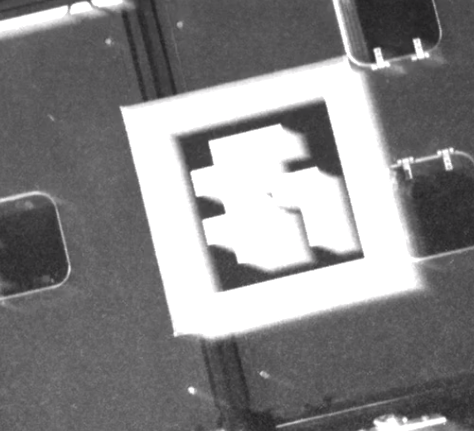
\includegraphics[width=.45\linewidth]{img/image_in_motion.png}
    \caption{Image from the onboard camera affected by motion blur}{Image from the onboard camera affected by motion blur due to high angular velocity of the UAV}
    \label{fig:imageInMotion}
\end{figure}

A closeup of the estimated and measured north component of the landing pad velocity $\vect{v}^n_{l/n,n}$ is given in figure~\ref{fig:dynamic_7_vel_closeup}.
\begin{figure}[!ht]
	\centering
	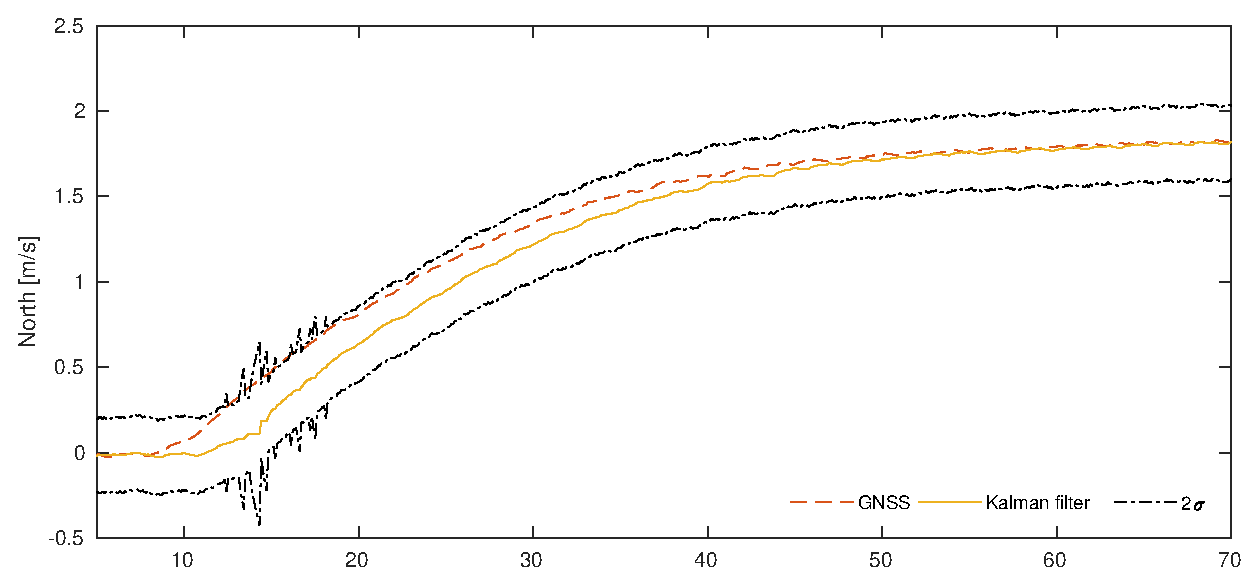
\includegraphics[width=.9\linewidth]{img/plot/dynamic/dynamic_7_vel_closeup.eps}
	\caption{Delay between the measured and estimated LP velocity}{Delay between the measured and estimated north component of the LP velocity}
	\label{fig:dynamic_7_vel_closeup}
\end{figure}
As the figure illustrates, there is a time delay of approximate 3 seconds between the changes in the measured velocity and the estimates velocity. This may be caused by the constant velocity model used in the Kalman filter equation derived in section \ref{sec:stateEstimation}. To be able to have a more accurate track of the landing pads during acceleration, the Kalman filter can be extended to a constant acceleration model. 

\subsection{Summary} % (fold)
\label{sub:kf_summary}
Since there is no precise reference measurements in the dataset, such as records from a motion capture lab or like, there is no straight forward method to validate the state estimates. However, from the figures in \ref{fig:kalmanTuningStaticTotal} and \ref{fig:kalmanTuningDynamic7} it can be seen that the Kalman filter is able to return smooth and reasonable state estimates. Moreover, several dozens of tests have been conducted in varying weather conditions such as windy, windless, snow, bright sun and cloudy. These tests have proven the state estimator to be robust and generate reliable and accurate navigation estimates.

Moreover, on static landing pads, the sensor bias estimated by the state estimator does include the position offset between the fiducial marker and the \gls{GNSS} receiver. Hence, the local navigation unit can be placed at an arbitrary place near by the landing pad and the position offset will automatically be included in the bias. 
% subsection summary (end)
%Delay in the velocity measurements due to constant velocity estimate.
% section state_estimator_tuning (end)